\documentclass[10pt,twocolumn]{article}

\usepackage[preprint]{neurips_2025}
\usepackage[T1]{fontenc}
\usepackage{amsmath}
\usepackage{amssymb}
\usepackage{booktabs}
\usepackage{array}
\usepackage{siunitx}
\sisetup{table-number-alignment=center, table-format=2.2}
\usepackage{enumitem}
\usepackage{float}
\usepackage{graphicx}
\graphicspath{{./}{../../}}
\usepackage{hyperref}
\usepackage{xcolor}
\usepackage{caption}
\usepackage{tikz}
\usetikzlibrary{arrows.meta, shapes.geometric, positioning, fit, backgrounds}
\usepackage{dblfloatfix}

\hypersetup{
  colorlinks=true,
  linkcolor=blue!50!black,
  citecolor=blue!50!black,
  urlcolor=blue!50!black
}

\captionsetup{
  font=footnotesize,
  labelfont=bf
}
\setlength{\columnsep}{0.25in}
\raggedbottom

\title{\textbf{Systematic Evaluation of Control Mechanisms for Factor-Based Portfolio Management}}
\author{Ioan Hedea}
\date{}

\begin{document}
\twocolumn[
\maketitle
\begin{abstract}
Portfolio management systems often separate alpha generation from risk control,
but the question of which control mechanism works best remains underexplored.
This paper systematically compares 13 control approaches over a finance-first
alpha engine built from factor, GARCH, and HMM sleeves, using frozen-bundle
evaluation across 77 traded tickers and 13 years of daily data from April 2013
through March 2026. The compared methods include no control beyond the factor
book, fixed exposure, simple rules, ensemble rules, contextual bandits,
supervised control, CVaR-aware robust optimization, and Q-learning RL. Results
show that CVaR-aware robust optimization has the strongest point estimates
among the tested controllers, achieving mean Sharpe 0.81 versus 0.40 for the
factor-only baseline, 0.42 for LinUCB, 0.41 for regime-aware rules, and 0.34
for RL; the best single run reaches 20.68\% annualized return with 0.91
Sharpe. Simple
regime-aware rules emerge as the strongest practical baseline, while the
learning-based approaches remain mixed. The supported conclusion is therefore
not that learning is the preferred control layer, but that systematic
controller comparison is the right research question and that, in this frozen
bundle, uncertainty-aware robust optimization is the most defensible control
mechanism.
\end{abstract}

\medskip
\noindent\textbf{Keywords:} portfolio management, factor investing, control mechanisms, robust optimization, contextual bandits, reinforcement learning, backtesting
]

\section{Introduction}

Many quantitative trading systems are modular long before they are learned.
Cross-sectional factors, volatility estimates, regime filters, and constrained
allocators already encode a large amount of domain structure before any control
policy is added. The practical question, then, is not only how to forecast
returns, but how much control complexity is justified once a finance-first
alpha engine is already working. Fixed allocation, simple rules, contextual
bandits, supervised controllers, robust optimization, and RL are all plausible
answers to that question.

The present manuscript reflects a deliberate architecture revision. Earlier
project versions were framed around whether RL worked as a controller. The
March 29, 2026 frozen-bundle evaluation broadened that question into a direct
comparison of control mechanisms. The resulting architecture keeps the proven
alpha core, factor anchoring, and constrained allocator, but evaluates a wider
set of downstream controllers under one shared data, timing, and cost protocol.

The revised implementation contributes five practical elements to the evaluation
setup.
\begin{enumerate}[leftmargin=1.5em, itemsep=2pt, topsep=4pt]
\item A modular code architecture that cleanly separates data, alpha, control,
      backtesting, and visualization concerns.
\item A factor-anchored alpha layer limited to components that survived pruning:
      cross-sectional factors, GARCH volatility forecasts, and a two-state HMM
      regime sleeve.
\item A constrained optimization layer between alpha and control that turns
      signals into a capped, turnover-aware, and group-aware target book.
\item A control-method comparison spanning fixed exposure, simple rules,
      contextual bandits, supervised control, robust optimization, and RL
      comparators.
\item A frozen-bundle research workflow including ablations, rolling windows,
      significance tests, reward sweeps, and regime-conditioned diagnostics.
\end{enumerate}

\subsection{Research Questions}

The current version of the report is organized around three revised research
questions.
\begin{enumerate}[leftmargin=1.5em, itemsep=2pt, topsep=4pt]
\item \textbf{RQ1: Control-method comparison.} Given a strong finance-first
      alpha engine, which controller adds the most value?
\item \textbf{RQ2: Competitive simple control.} Can simple rules provide
      competitive downside control without excessive Sharpe degradation?
\item \textbf{RQ3: Learning versus optimization.} Do learning-based methods
      outperform optimization-based control on top of the same alpha engine?
\end{enumerate}

From a research perspective, this framing matters because it narrows the gap
between a teaching prototype and a system that can be discussed in the language
of quantitative portfolio construction. The objective is not to claim that the
pipeline is production-ready. Rather, it is to assemble a well-motivated stack
in which each modeling choice has a clear financial role and where performance
can be decomposed into alpha generation, portfolio construction, and control.

The central defended statement is therefore not that a specific learning method
wins. It is that a finance-first alpha engine should be paired with a
systematic controller comparison under explicit timing and cost assumptions.
The finished frozen bundle shows that robust optimization currently provides
the strongest control outcome, that simple regime-aware rules are already
competitive, and that the learning-based methods in this study do not beat the
best optimization-based approach.

\section{Related Literature and Design Motivation}

The report is not meant to claim novelty in any individual modeling choice.
Instead, it builds a coherent pipeline from well-established ingredients.

\textbf{Factor investing.} The cross-sectional component is aligned with the idea
that common risk factors help explain returns \cite{fama1993}. Momentum is
motivated by the medium-horizon continuation evidence of Jegadeesh and Titman
\cite{jegadeesh1993}, while quality and low-volatility proxies are included to
stabilize the cross-section.

\textbf{Volatility and regimes.} Conditional heteroskedasticity motivates the
GARCH sleeve \cite{engle1982,bollerslev1986}, while the market-regime component
uses a two-state hidden Markov model in the spirit of Hamilton \cite{hamilton1989}.

\textbf{Rule-based, bandit, and optimization-based control.} A key part of the
revised paper is that RL is no longer the only sophisticated controller under
study. Volatility targeting, drawdown-based deleveraging, regime rules,
contextual bandits, supervised controllers, and CVaR-aware robust allocation
are all treated as serious alternatives because these are the kinds of methods
one would compare before concluding that sequential RL is necessary.

\textbf{Reinforcement learning.} RL is used as a controller rather than a raw
alpha generator. This follows the practical observation that in finance, RL is
often most useful for allocation, inventory, and execution decisions rather than
for replacing domain-specific signal construction \cite{sutton2018,almgren2000}.
This role assignment is also motivated by the low signal-to-noise ratio and
limited effective sample size typical of financial data, which make end-to-end
policy learning especially brittle.

\subsection{Recent Work on RL for Portfolio Management}

Recent work on RL in portfolio management and trading can be organized into four
overlapping strands.

\textbf{End-to-end policy learning.} Early and influential work uses RL to learn
trading or allocation policies directly from price histories and realized
rewards \cite{moody2001,deng2017,jiang2017,zhang2020,cong2021,pacheco2023}. The appeal of
this approach is conceptual elegance: the same learner is asked to extract
signal, size positions, and adapt sequentially. The difficulty is that
financial returns are noisy, nonstationary, and data-poor relative to many
other machine-learning domains. As a result, end-to-end RL systems can be
sample-inefficient, regime-sensitive, and hard to interpret when they fail
\cite{gu2020,kolm2019,jander2025}.

\textbf{Neural return forecasting with a separate optimizer.} A second line of
work uses deep or other machine-learning models to estimate returns, factors, or
pricing kernels, then hands those forecasts to a conventional optimizer
\cite{gu2020,chen2021,giglio2022}. This preserves more structure in the
allocation step than end-to-end RL, and often performs well empirically, but it
still concentrates modeling risk in a data-hungry prediction layer.

\textbf{RL for execution and risk control.} A third strand applies RL to
narrower sequential tasks such as execution and dynamic risk management rather
than to raw alpha discovery \cite{nevmyvaka2006,kolm2019hedge,buehler2019,du2020}.
This decomposition is closest to the present paper. The core idea is that RL
may be most useful where the problem is inherently sequential and control-like,
while alpha generation remains anchored to domain models or explicit financial
structure.

\textbf{Benchmarking and reproducibility.} More recent platform and survey work
has emphasized that RL in finance still suffers from weak evaluation discipline,
narrow datasets, and inconsistent reporting \cite{sun2023,jander2025}. That
critique directly motivates the frozen-bundle methodology used here.

Table~\ref{tab:taxonomy} positions the present approach relative to these
broader families. The contribution is not a new RL algorithm. It is a
methodological proposal: if strong finance-first alpha already exists, the main
research question should be a disciplined comparison of control mechanisms, with
RL judged against simple rules and end-to-end learned alternatives rather than
against passive exposure alone.

\begin{table*}[t]
\centering
\scriptsize
\caption{Taxonomy of portfolio-management architectures.}
\label{tab:taxonomy}
\begin{tabular}{@{} >{\raggedright\arraybackslash}p{2.1cm}
                >{\raggedright\arraybackslash}p{2.1cm}
                >{\raggedright\arraybackslash}p{2.15cm}
                >{\raggedright\arraybackslash}p{1.45cm}
                >{\raggedright\arraybackslash}p{4.2cm} @{}}
\toprule
\textbf{Approach} & \textbf{Alpha source} & \textbf{Control logic} & \textbf{Interp.} & \textbf{Representative references} \\
\midrule
Classical factors & Hand-crafted financial signals & Fixed allocator or simple overlay rules & High & Fama--French style factor investing \cite{fama1993} \\
Rule-based overlays & Finance-first alpha models & Vol-targeting, deleveraging, and exposure rules & High & Simple portfolio-risk overlays in practice \cite{almgren2000} \\
End-to-end RL & Learned from market histories & RL policy directly selects positions or weights & Low to medium & Direct trading and portfolio RL \cite{moody2001,jiang2017,zhang2020,cong2021} \\
Neural forecasting + optimizer & Neural or ML return forecasts & Separate optimizer translates forecasts into holdings & Medium & Asset-pricing and return-forecast models \cite{gu2020,chen2021,giglio2022} \\
\textbf{This paper} & \textbf{Finance-first alpha models} & \textbf{Comparison of rule-based, bandit, supervised, robust, and RL control} & \textbf{High} & \textbf{Frozen-bundle control-method evaluation} \\
\bottomrule
\end{tabular}
\end{table*}

\subsection{Contribution Type}

The contribution is not novelty in any single alpha ingredient. The paper does
not claim a new factor model, a new GARCH variant, or a new RL algorithm. Its
contribution lies instead in three places. First, it proposes a clear role
assignment between alpha and control: financially grounded models produce the
alpha book, while controllers decide how aggressively to express it. Second, it
implements that role assignment in a modular architecture with an explicit
constrained allocator between alpha and control. Third, it pairs the
architecture with a frozen-bundle evaluation workflow designed to test that
claim via ablations, timing-discipline checks, robustness slices, significance
tests, and regime-conditioned behavior summaries. The contribution is therefore
chiefly methodological: the paper proposes and tests a disciplined way to
evaluate portfolio control mechanisms on top of a finance-first alpha engine.

\section{System Architecture}

The pipeline is organized as a linear sequence of stages, illustrated in
Figure~\ref{fig:architecture}. Upstream stages produce signals and risk
features, the allocator turns those signals into a target book, and the control
layer decides how much of that book to express before the backtest engine
records realized outcomes.

\begin{figure*}[t]
\centering
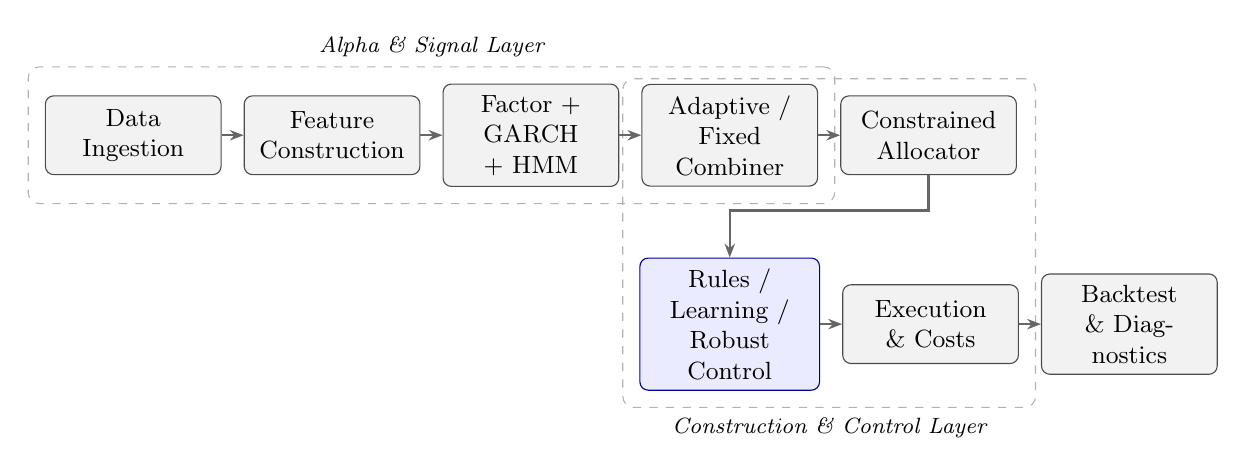
\begin{tikzpicture}[
  node distance = 0.45cm and 0.28cm,
  box/.style = {
    rectangle, rounded corners=3pt,
    draw=black!70, fill=gray!10,
    text width=1.95cm, align=center,
    font=\small, minimum height=1.0cm,
    inner sep=4pt
  },
  rlbox/.style = {
    rectangle, rounded corners=3pt,
    draw=blue!60!black, fill=blue!8,
    text width=2.0cm, align=center,
    font=\small, minimum height=1.0cm,
    inner sep=4pt
  },
  arr/.style = {-{Stealth[length=5pt]}, thick, black!60},
  groupbox/.style = {
    draw=black!30, dashed, rounded corners=4pt,
    fill=none, inner sep=6pt
  }
]
\node[box] (data)    {Data\\Ingestion};
\node[box, right=of data]    (feat)    {Feature\\Construction};
\node[box, right=of feat]    (alpha)   {Factor +\\GARCH + HMM};
\node[box, right=of alpha]   (comb)    {Adaptive /\\Fixed Combiner};
\node[box, right=of comb]    (alloc)   {Constrained\\Allocator};
\node[rlbox, below=0.9cm of comb] (control) {Rules / Learning /\\Robust Control};
\node[box, right=of control] (exec)    {Execution\\\& Costs};
\node[box, right=of exec]    (bt)      {Backtest\\\& Diagnostics};

\draw[arr] (data)  -- (feat);
\draw[arr] (feat)  -- (alpha);
\draw[arr] (alpha) -- (comb);
\draw[arr] (comb)  -- (alloc);
\draw[arr] (alloc.south) -- ++(0,-0.45) -| (control.north);
\draw[arr] (control) -- (exec);
\draw[arr] (exec) -- (bt);

\begin{scope}[on background layer]
  \node[groupbox, fit=(data)(feat)(alpha)(comb),
        label={[font=\footnotesize\itshape]above:Alpha \& Signal Layer}] {};
  \node[groupbox, fit=(alloc)(control)(exec),
        label={[font=\footnotesize\itshape]below:Construction \& Control Layer}] {};
\end{scope}
\end{tikzpicture}
\caption{High-level architecture of the revised quantitative trading pipeline.
The alpha layer is intentionally finance-first, the allocator builds a capped
and turnover-aware target book, and the control comparison focuses on how much
of that book to express rather than on a second stock-selection problem. The
compared control families span simple rules, contextual bandits, supervised
control, robust optimization, and RL.}
\label{fig:architecture}
\end{figure*}

\subsection{Software Structure}

Table~\ref{tab:modules} summarizes the package decomposition that supports the
frozen-bundle workflow. The separation is intentional: alpha construction,
control comparison, backtesting, and plotting are kept in distinct modules so
that the reported artifact bundle can be regenerated and audited component by
component.

\begin{table*}[t]
\centering
\caption{Module-level decomposition of the \texttt{quant\_stack} package.}
\label{tab:modules}
\small
\begin{tabular}{@{} l p{0.78\textwidth} @{}}
\toprule
\textbf{Module} & \textbf{Responsibility} \\
\midrule
\texttt{config.py}   & Universe definition, global constants, and external series identifiers \\
\texttt{data.py}     & Market price/volume ingestion, macro series (FRED / BLS fallback), and SEC company facts \\
\texttt{alpha.py}    & Cross-sectional factors, GARCH volatility, HMM regime, and adaptive or fixed signal combination \\
\texttt{rl.py}       & Portfolio controller, state construction, and end-to-end PPO benchmark interfaces \\
\texttt{pipeline.py} & Walk-forward backtest orchestration and online RL update loop \\
\texttt{evaluation.py} & Control-method comparison, ablation, rolling-window robustness, significance tests, and artifact export \\
\texttt{plots.py}    & Equity-curve, drawdown, controller-behavior, robustness, and reward-ablation figures \\
\texttt{main.py}     & CLI entry point and compatibility wrapper \\
\bottomrule
\end{tabular}
\end{table*}

\section{Data and Feature Construction}

\subsection{Universe}

The revised frozen bundle uses the expanded universe rather than the smaller
development basket. It contains 77 traded tickers spread across technology,
financials, healthcare, consumer staples, energy, industrials, materials, real
estate, utilities, communications, consumer discretionary, and diversifier
exposures such as GLD, TLT, and VNQ. SPY serves as the passive equity benchmark
throughout.

\subsection{Data Sources}

Daily prices and volumes are sourced via \texttt{yfinance}. When a
\texttt{FRED\_API\_KEY} is available, macro data are drawn directly from FRED;
in its absence, the system falls back to BLS and U.S.\ Treasury Fiscal Data.
SEC company facts are incorporated when \texttt{SEC\_USER\_AGENT} is set,
enabling a light fundamentals layer without requiring a proprietary data
subscription.

\subsection{Macro Regime Inputs}

When available, the macro sleeve includes the 10-year yield, 2-year yield,
federal funds rate, unemployment rate, and term spread. The updated research
design also incorporates stress-sensitive FRED series including the VIX, the
ICE BofA high-yield option-adjusted spread, and a dollar-index proxy. These
variables do not form a standalone alpha book. Instead, they help create a
macro regime belief that is blended with the HMM regime estimate and provide
additional context for risk-off states.

\subsection{Information-Timing Contract}

One of the most important research upgrades in the current version is that the
pipeline makes its feature-availability assumptions explicit. Macro inputs are
shifted forward by a configurable number of trading days before they are allowed
into the backtest. This is still weaker than a true real-time vintage database,
because it does not model revisions, but it is materially stronger than using
the final macro history with no delay assumption at all.

Fundamental inputs are handled more conservatively. The SEC quality signal is
still a static cross-sectional research prior rather than a fully point-in-time
fundamentals panel. For that reason the research engine supports a strict timing
mode in which the SEC quality sleeve is disabled and macro inputs are forced to
use the largest configured lag. The point of this design is not to pretend that
point-in-time fundamentals are already solved, but rather to make the timing
caveat measurable and visible in the evaluation workflow.

\section{Methodology}

\subsection{Problem Formulation}

Let $r_{t+1} \in \mathbb{R}^N$ denote next-period asset returns for a universe of
$N$ tradable assets. At time $t$, the system observes a feature state
$x_t \in \mathcal{X}$ constructed from cross-sectional factor values,
volatility forecasts, regime beliefs, macro inputs, recent portfolio returns,
and allocation summaries. The alpha layer maps these features into an
expected-return score vector $\alpha_t \in \mathbb{R}^N$ and a confidence
vector $c_t \in \mathbb{R}^N$.

The control layer then chooses a portfolio allocation $w_t$ and a cash
allocation. The one-step objective is not written as a pure return-maximization
problem. Instead, it is implicitly multi-objective: maximize long-run wealth
while limiting drawdown, volatility, and unnecessary turnover. This is the
reason the project separates alpha estimation from control: the two tasks
operate on different time scales and carry different inductive biases.
Importantly, the learned controller does not forecast $r_{t+1}$ directly; it
maps a state summarizing alpha opportunity, current allocation, and recent
portfolio outcomes into exposure and overlay decisions.

\subsection{Cross-Sectional Factor Model}

The factor sleeve combines four z-scored components: momentum, a value proxy, a
quality proxy, and a low-volatility tilt. Letting $m_i$, $v_i$, $q_i$, and
$\ell_i$ denote the standardized scores for asset $i$, the composite factor
score is
\[
f_i = 0.30 m_i + 0.25 v_i + 0.25 q_i + 0.20 \ell_i.
\]
This choice reflects a balanced, multi-style factor book rather than a single
directional bet. In the revised architecture, this factor book is the dominant
alpha source, with the other retained sleeves acting mainly as stabilizers or
confidence modifiers rather than as separate return engines.

\subsection{Volatility and Regime Models}

Each name receives a GARCH(1,1) forecast
\[
\sigma_t^2 = \omega + \alpha_1 \epsilon_{t-1}^2 + \beta_1 \sigma_{t-1}^2,
\]
where $\omega > 0$, $\alpha_1 \geq 0$, and $\beta_1 \geq 0$ are the intercept,
ARCH, and GARCH coefficients respectively. This conditional variance estimate
is used for confidence scaling and risk awareness. Separately, a two-state HMM
produces a bull-versus-bear regime belief. The final regime signal is
\[
\text{RegimeBelief}_t =
0.75 \cdot \text{HMMBelief}_t +
0.25 \cdot \text{MacroBelief}_t.
\]

\subsection{Adaptive Alpha Combination}

Let $s^{(k)}_{i,t}$ denote the signal from source $k$ for asset $i$ at time $t$.
The expected return score is formed as
\[
\alpha_{i,t} = \sum_k w^{(k)}_t s^{(k)}_{i,t},
\]
where the source weights $w^{(k)}_t$ adapt over time based on recent realized
signal quality. In the implementation, this is proxied by recent Spearman
information coefficients between source scores and realized returns.

This adaptive weighting is important because the retained sleeves are not
equally informative across all market states. In the revised architecture,
however, adaptive weighting is explicitly treated as an ablation rather than as
an article of faith. Fixed weights remain a strong baseline precisely because
the root-level bundle suggests that adaptive combination does not obviously add
value in the current sample.

\subsection{Constrained Allocator}

The controller is not handed raw scores and asked to build a book from scratch.
Instead, the revised architecture inserts a constrained intermediate allocator
between the alpha layer and the control layer. The factor-anchored target book
is
\[
w_t^{\text{target}} =
0.90\,w_t^{\text{factor}} +
0.10\,w_t^{\text{stabilizer}},
\]
where the stabilizer is a long-only minimum-variance-style portfolio estimated
from a Ledoit--Wolf shrinkage covariance matrix.

The allocator solves a small regularized problem of the form
\[
\min_w \quad
\lambda_{\mathrm{risk}} w^\top \Sigma_t w
- \lambda_{\alpha}\alpha_t^\top w
+ \lambda_{\mathrm{anchor}}\lVert w - w_t^{\mathrm{target}} \rVert_2^2
+ \lambda_{\mathrm{turn}}\lVert w - w_{t-1} \rVert_2^2
\]
subject to $w_i \ge 0$, $\sum_i w_i = 1$, per-asset caps, and group
concentration limits. This intermediate layer is not only an architectural
convenience; it reflects the practical fact that many real portfolio systems
mediate between forecast signals and final positions through a constrained
allocator.

\subsection{Control Methods}

The completed frozen bundle compares five families of control methods built on
the same finance-first alpha engine and constrained allocator.
\begin{enumerate}[leftmargin=1.5em, itemsep=2pt, topsep=4pt]
\item \textbf{Alpha and fixed-rule baselines.} The suite includes
      \texttt{factor\_only}, a fixed 95\% allocator, volatility targeting,
      drawdown-based deleveraging, regime-aware rules, and simple rule
      ensembles.
\item \textbf{Contextual bandits.} Three lightweight bandit controllers are
      evaluated: LinUCB, Thompson sampling, and an $\varepsilon$-greedy linear
      controller.
\item \textbf{Supervised control.} An expanding-window classifier predicts the
      most attractive exposure bucket from the same compact state summary.
\item \textbf{Robust optimization.} A CVaR-aware robust allocator augments the
      constrained optimizer with downside-sensitive risk control and is the
      main non-learning advanced comparator.
\item \textbf{RL comparators.} Tabular portfolio Q-learning remains as a direct
      learned-controller baseline, and end-to-end PPO is retained as a
      monolithic comparator outside the main control-comparison suite.
\end{enumerate}

\subsection{Portfolio RL}

The revised portfolio RL state is deliberately minimal. It is constructed from
the current alpha-score cross-section, the current portfolio-weight summary, and
recent portfolio returns. This pruned state replaces the richer regime,
uncertainty, volatility, and hedge-specific state variables used in the older
architecture.

If the RL agent chooses invested fraction $b_t$ and active overlay size $\tau_t$,
the final invested portfolio is approximately
\[
w_t =
b_t \left[(1-\tau_t)w_t^{\text{target}} + \tau_t w_t^{\text{satellite}}\right].
\]
The satellite sleeve is not a fully independent book; it tilts the factor target
toward the strongest alpha names. This keeps the full pipeline close to the
working factor engine while still letting RL modulate aggressiveness.

\subsection{Reward Design}

The revised architecture uses a Sortino-style reward by default. In compact
form,
\[
R_t^{\mathrm{portfolio}}
= \frac{r_t - \hat{\mu}_t}{\hat{\sigma}^{\mathrm{down}}_t + \varepsilon},
\]
where $\hat{\mu}_t$ is a running mean and
$\hat{\sigma}^{\mathrm{down}}_t$ is a running downside-deviation estimate. The
agent is therefore rewarded for improving return relative to downside risk
rather than for taking more total variance in absolute terms.

The research runner also supports reward-function ablations over
differential-Sharpe, raw-return, Sortino, and mean-variance formulations. This
matters because reward design is one of the least observable but most important
degrees of freedom in RL-for-finance systems. Because reward specification
changes the controller's operating point, it should be treated as a
methodological degree of freedom rather than as a neutral implementation detail.

\subsection{No-Trade Band and Transaction Costs}

To reduce turnover drag, a rebalance band suppresses small changes in target
weights. When only part of the portfolio is changed, the active weights are
rescaled to preserve the desired capital budget.

The backtest includes a three-part execution-cost approximation. For each
rebalance, the strategy pays a fixed basis-point fee on turnover, an additional
penalty proportional to turnover times realized volatility, and a size penalty
linked to the largest one-name weight change. In symbols,
\[
\mathrm{TC}_t
= c_0 \cdot \mathrm{turnover}_t
+ c_1 \cdot \mathrm{turnover}_t \cdot \hat{\sigma}_t
+ c_2 \cdot \max_i |\Delta w_{i,t}|.
\]
This is not a full execution simulator, but it pushes the daily allocator away
from unrealistic churn and makes the rebalance band economically meaningful
rather than purely cosmetic.

\section{Experimental Design}

The revised frozen bundle used in the paper contains 3{,}269 daily observations
from April 1, 2013 through March 27, 2026. The completed root-level bundle
contains 78 runs spanning legacy ablations, 13 control-method candidates across
three train fractions, a strict-timing check, six rolling windows, four cost
settings, three rebalance-band settings, three macro-lag settings, four reward
settings, and five blocked time-series CV folds. The manuscript is tied to the
resulting root-level artifacts, especially \texttt{research\_summary.json},
\texttt{research\_control\_comparison.csv}, and the companion CSV and PNG
outputs. This does not eliminate prior exploratory iteration, but it does make
the reported bundle explicit and reproducible.

Within that archived suite, action ladders, optimizer settings, reward choices,
and comparison baselines are held fixed across ablations, split-fraction tests,
rolling-window robustness slices, and significance calculations. The control
comparison itself uses train fractions \{0.4, 0.5, 0.6\} and evaluates
factor-only, fixed allocation, rule-based control, contextual bandits,
supervised control, CVaR-aware robust optimization, and RL under the same cost
and timing discipline.

At each date, the revised pipeline executes the following sequence. First,
factor, GARCH, HMM, macro, and optional SEC features are generated from the
available data. These are combined into expected-return scores via either the
adaptive or fixed combiner. The constrained allocator produces the target book.
The chosen controller then decides how much of that book to express via
invested fraction and active overlay size. Transaction costs and cash carry are
applied to arrive at the realized portfolio return, which is finally used to
update the RL value table when the controller is learned.

\subsection{Benchmark Logic}

The benchmark set is chosen to isolate different sources of value. SPY measures
whether the pipeline adds value relative to standard passive equity exposure.
The factor-only benchmark isolates the pure alpha layer without any controller
overlay. Because the archived bundle already uses a broad 77-ticker universe,
this factor benchmark is also informative about what the diversified opportunity
set can do without learned control. Comparing the full pipeline against the
factor-only benchmark is particularly important because it reveals whether
learning is adding value as a controller or merely acting as a drag on a strong
signal engine.

The newer comparison baselines sharpen that logic further. The volatility
targeting baseline asks whether most of the observed improvement can be matched
by simple inverse-vol scaling. The drawdown-based deleveraging baseline asks
whether a threshold rule can replicate the control layer's protection effect.
The end-to-end PPO baseline addresses the paper's most distinctive
architectural question: if one hands the same state information to a monolithic
policy, does it outperform a hybrid design in which finance-specific modules
produce the target book and RL only controls how aggressively to express it?
These baselines are deliberately strong because they represent the kinds of
simple overlays a practitioner would try before accepting the complexity of RL.

\section{Evaluation Metrics}

The reporting suite includes annualized return, annualized volatility, Sharpe
ratio, Sortino ratio, maximum drawdown, Calmar ratio, and return-distribution
diagnostics including a daily 5\% Value-at-Risk estimate.

If $\{r_t\}_{t=1}^T$ denotes daily portfolio returns and $r_f$ is the annual
risk-free rate, then the annualized Sharpe ratio is
\[
\text{Sharpe} = \frac{252 \, \bar{r} - r_f}{\sqrt{252}\,\hat{\sigma}(r) + \varepsilon}.
\]
The Sortino ratio replaces total volatility with downside volatility, while the
Calmar ratio scales annualized return by the magnitude of maximum drawdown. Each
metric emphasizes a different aspect of the return distribution, which matters
in this project because the controller is explicitly designed to reshape risk,
not merely to maximize mean return. Table~\ref{tab:metrics} focuses on the
primary comparison metrics used in the main strategy table: return, volatility,
Sharpe, maximum drawdown, and Calmar. Sortino and Value-at-Risk are retained as
secondary diagnostics in the text, reward-ablation evidence, and archived
research artifacts.

\section{Results}

This section first reports the new control-comparison headline, then uses the
legacy ablation and full-pipeline diagnostics as secondary evidence about which
sources of complexity were worth keeping. The key change relative to earlier
drafts is that the paper no longer treats RL as the protagonist. The main
question is which controller is strongest on top of the same finance-first
alpha engine.

\subsection{Main Result: Control Comparison}

The main result is the completed 13-method control-comparison suite.
Table~\ref{tab:metrics} reports mean annualized performance across the three
train/test split settings used in the frozen bundle.

\begin{table*}[t]
\centering
\small
\caption{Control-comparison summary across train/test split settings. All
methods share the same finance-first alpha engine and constrained allocator.
Annualized figures.}
\label{tab:metrics}
\begin{tabular}{@{} l r r r r r @{}}
\toprule
\textbf{Controller} & \textbf{Return} & \textbf{Vol.} & \textbf{Sharpe} & \textbf{Max DD} & \textbf{Calmar} \\
\midrule
Factor-only baseline & 9.2\% & 13.4\% & 0.40 & $-$19.8\% & 0.46 \\
A1: Fixed & 9.0\% & 12.7\% & 0.40 & $-$18.6\% & 0.48 \\
A2: Vol-target & 6.9\% & 10.0\% & 0.34 & $-$13.3\% & 0.51 \\
A3: DD-Delever & 6.6\% & 11.7\% & 0.25 & $-$18.4\% & 0.36 \\
A4: Regime rules & 8.8\% & 11.9\% & 0.41 & $-$16.1\% & 0.54 \\
A5: Ensemble (mean) & 7.4\% & 11.5\% & 0.32 & $-$15.3\% & 0.48 \\
A5: Ensemble (min) & 6.6\% & 10.1\% & 0.30 & $-$12.7\% & 0.51 \\
B1: LinUCB & 9.0\% & 12.3\% & 0.42 & $-$18.0\% & 0.50 \\
B2: Thompson & 7.9\% & 12.3\% & 0.33 & $-$18.6\% & 0.42 \\
B3: Eps-greedy & 8.4\% & 12.3\% & 0.37 & $-$18.0\% & 0.46 \\
C: Supervised & 8.9\% & 12.5\% & 0.40 & $-$19.2\% & 0.45 \\
\textbf{D: CVaR-robust} & \textbf{17.6\%} & \textbf{17.3\%} & \textbf{0.81} & \textbf{$-$26.4\%} & \textbf{0.68} \\
RL: Q-learning & 7.9\% & 12.1\% & 0.34 & $-$18.3\% & 0.42 \\
\bottomrule
\end{tabular}
\end{table*}

As an external calibration point, SPY averages 14.0\% annualized return,
18.8\% volatility, 0.56 Sharpe, and $-$30.6\% maximum drawdown across the same
three control-comparison splits. It is not shown as a row in
Table~\ref{tab:metrics} because SPY is a passive benchmark rather than a
controller applied to the shared alpha engine. In that numerical sense,
CVaR-robust is the only controller in the study that is genuinely close to or
above SPY on both return and Sharpe.

The main answer to \textbf{RQ1} is clear: CVaR-aware robust optimization is the
strongest control mechanism in the completed suite. Its mean Sharpe of 0.81 is
well above the factor-only baseline at 0.40 and far above the learning-based
controllers. The best single run in the control-comparison suite,
\texttt{D\_cvar\_robust\_tf0.50}, reaches 20.68\% annualized return with 0.91
Sharpe.

The main answer to \textbf{RQ2} is also positive. Simple rules can provide
competitive risk control. In particular, regime-aware rules reach Sharpe 0.415
with maximum drawdown $-$16.1\%, improving on the factor-only baseline's 0.402
Sharpe and $-$19.8\% drawdown. Fixed allocation is similarly competitive, while
vol-targeting offers the best drawdown control among the simple rules at the
cost of lower return.

The main answer to \textbf{RQ3} is negative for the learning-based methods.
LinUCB is the best learner at Sharpe 0.424, slightly ahead of the factor-only
baseline and the better simple rules, but still far below the robust optimizer
at 0.81. The supervised controller reaches 0.395 Sharpe, and tabular
Q-learning reaches 0.342. In this finished bundle, the learning-based methods
do not beat the optimization-based approach.

One important qualification is statistical rather than economic. The archived
pairwise bootstrap table currently covers the legacy full pipeline versus
baselines, not the new controller-to-controller comparisons. The appropriate
claim in this section is therefore that CVaR-aware robust optimization is the
point-estimate leader, not yet a statistically settled winner over
regime-aware rules or LinUCB.

That point-estimate lead also comes with an important downside caveat:
CVaR-robust has the worst mean maximum drawdown in Table~\ref{tab:metrics} at
$-$26.4\%. This is not internally inconsistent, because the objective is
CVaR-aware rather than maximum-drawdown-minimizing: it penalizes tail losses in
the return distribution while still running at a materially higher average risk
budget to earn much higher return. In the current bundle it improves Sharpe and
Calmar, but not the single worst realized peak-to-trough path event. If maximum
drawdown is the primary mandate, regime-aware rules and volatility targeting
remain the more conservative choices.

\noindent\textit{Implication for the revised RQs.} \textbf{RQ1}: answered in
favor of CVaR-aware robust optimization. \textbf{RQ2}: answered positively,
with regime-aware rules providing a strong practical baseline. \textbf{RQ3}:
answered negatively for learning-based control; the best learner remains well
below the best optimization-based method.

\IfFileExists{../../control_method_overview.png}{
\begin{figure*}[t]
\centering
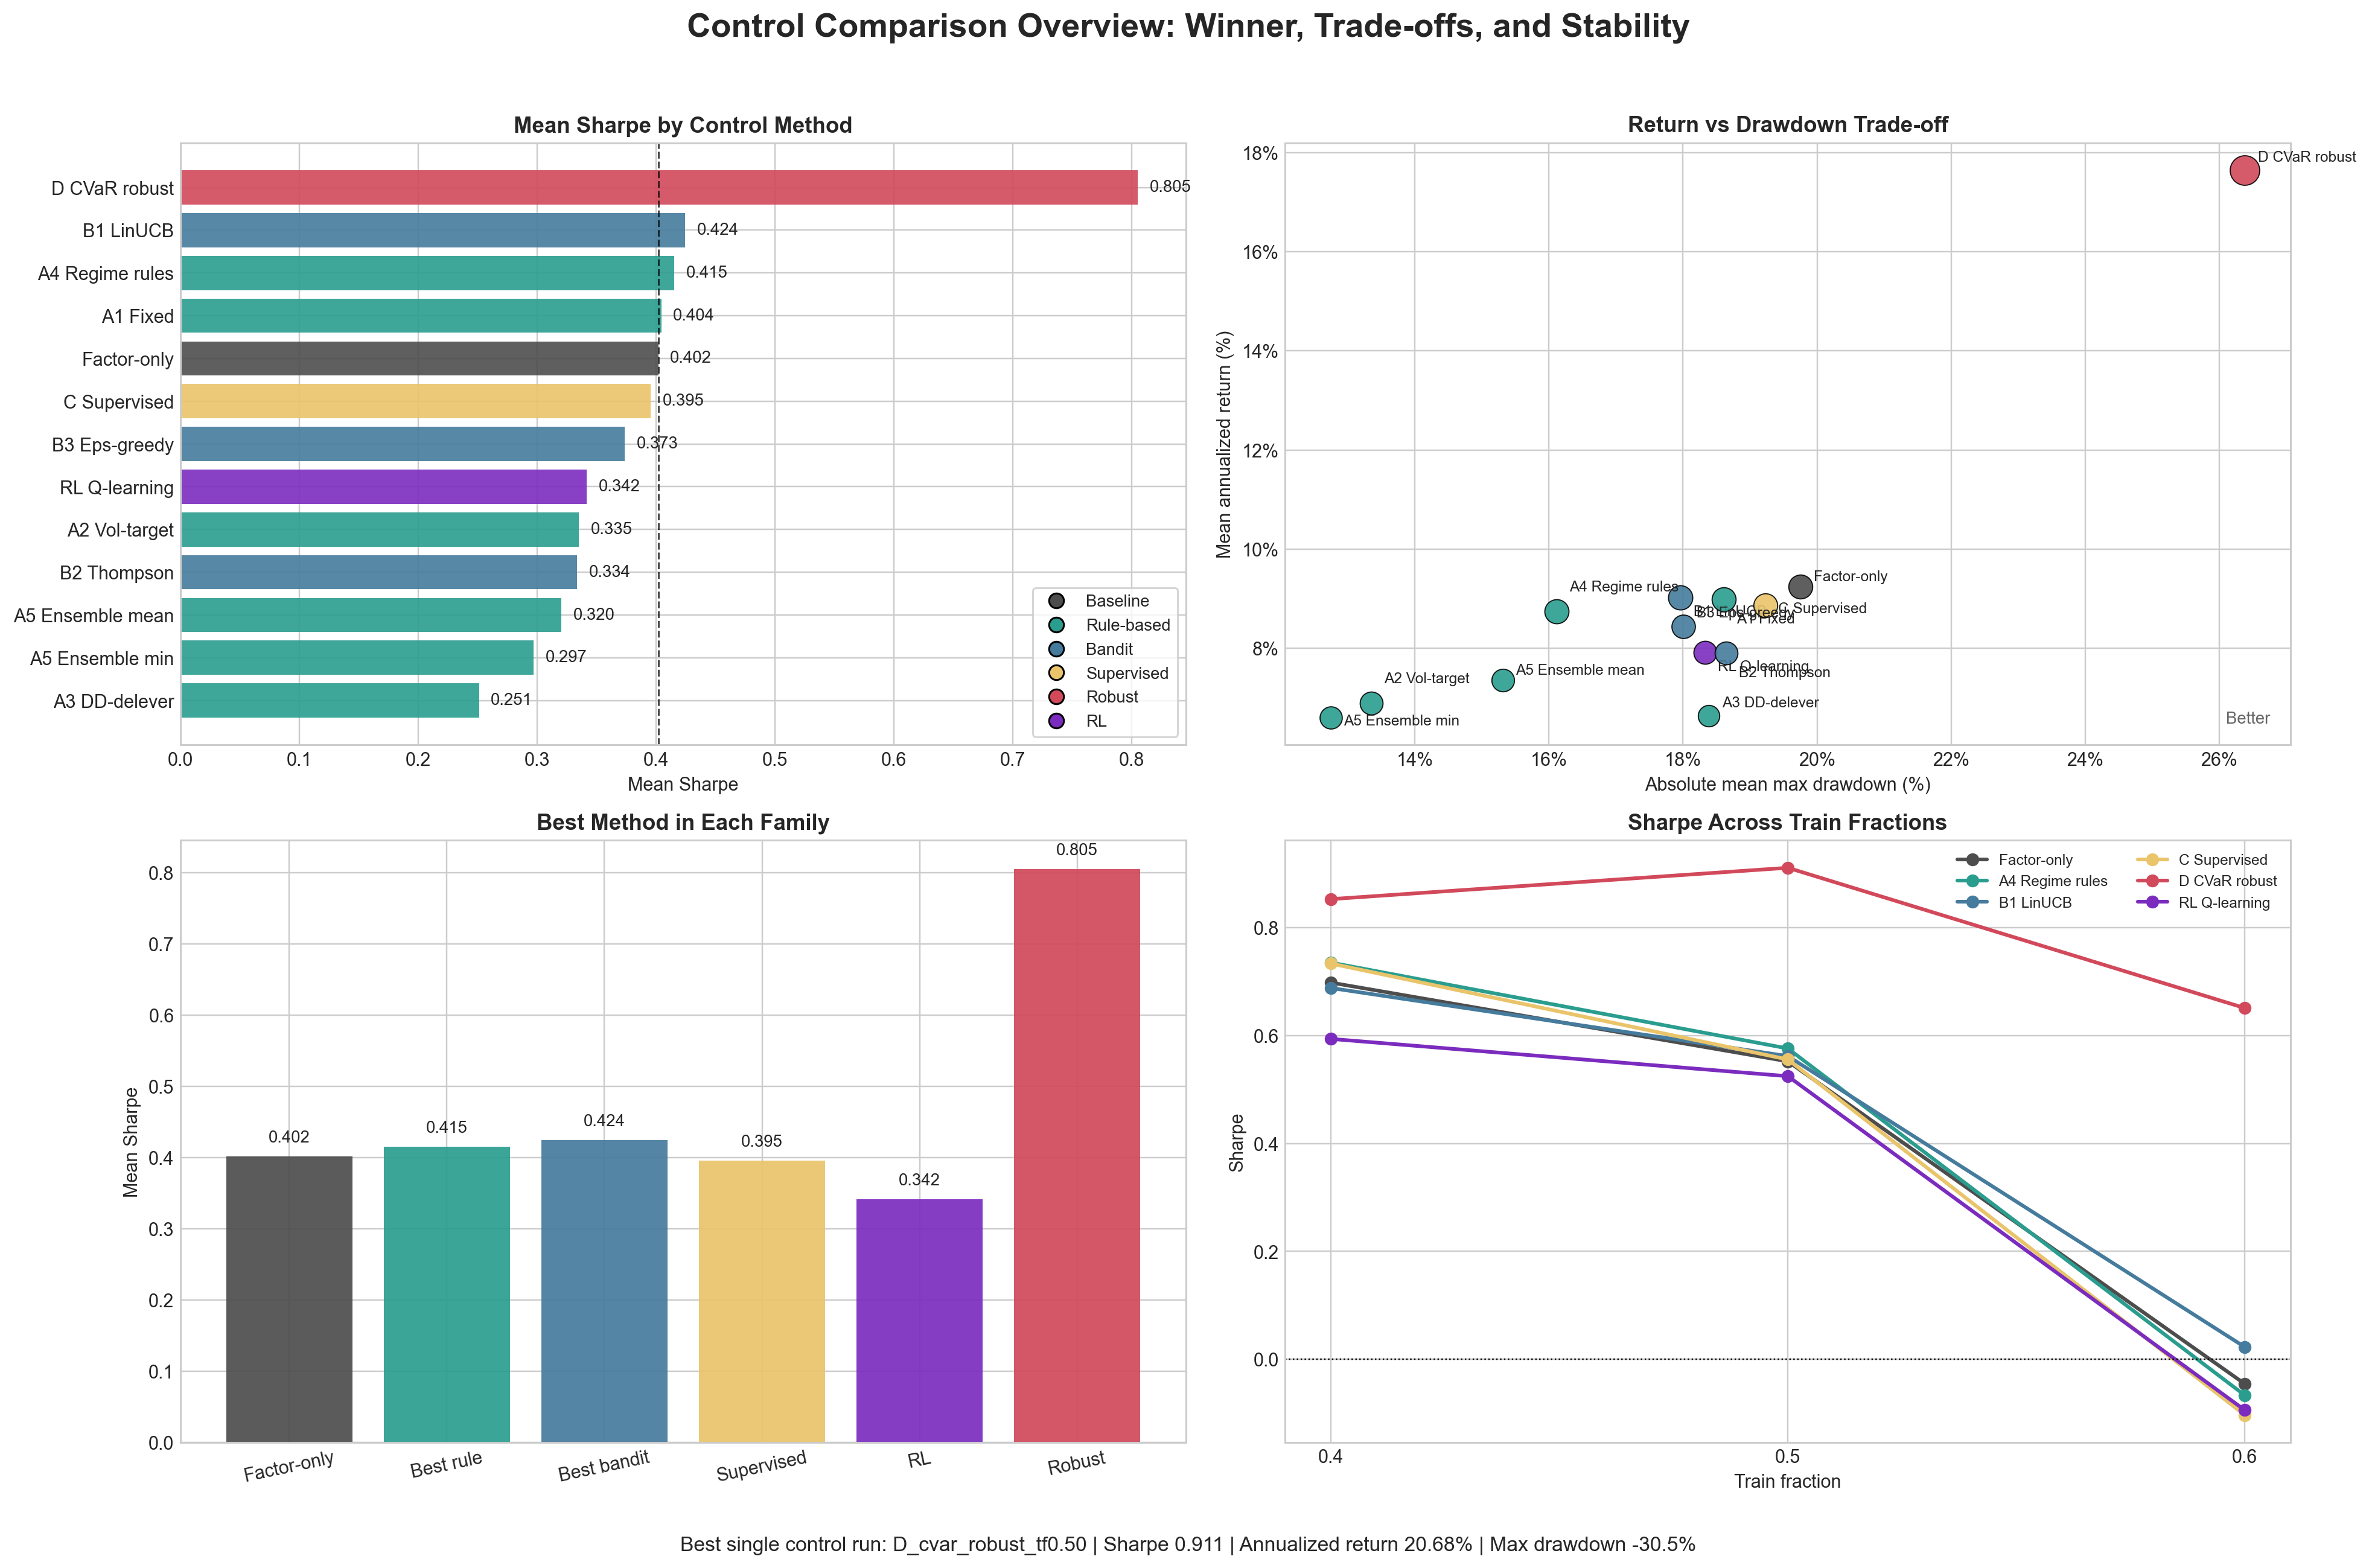
\includegraphics[width=\textwidth]{../../control_method_overview.png}
\caption{Overview of the finished control-comparison bundle. The panels show
the full ranking by mean Sharpe, return-versus-drawdown trade-offs, the best
representative in each controller family, and split-to-split Sharpe stability
for selected methods. The main visual message is that CVaR-aware robust
optimization is the strongest point-estimate controller in the new study, while
simple rules remain competitive and RL is not the leading method.}
\label{fig:control_overview}
\end{figure*}
}{
\noindent\textit{Research note.} When the dedicated research runner is executed,
it also emits a compact figure summarizing the control comparison.
}

\IfFileExists{../../control_split_heatmaps.png}{
\begin{figure*}[t]
\centering
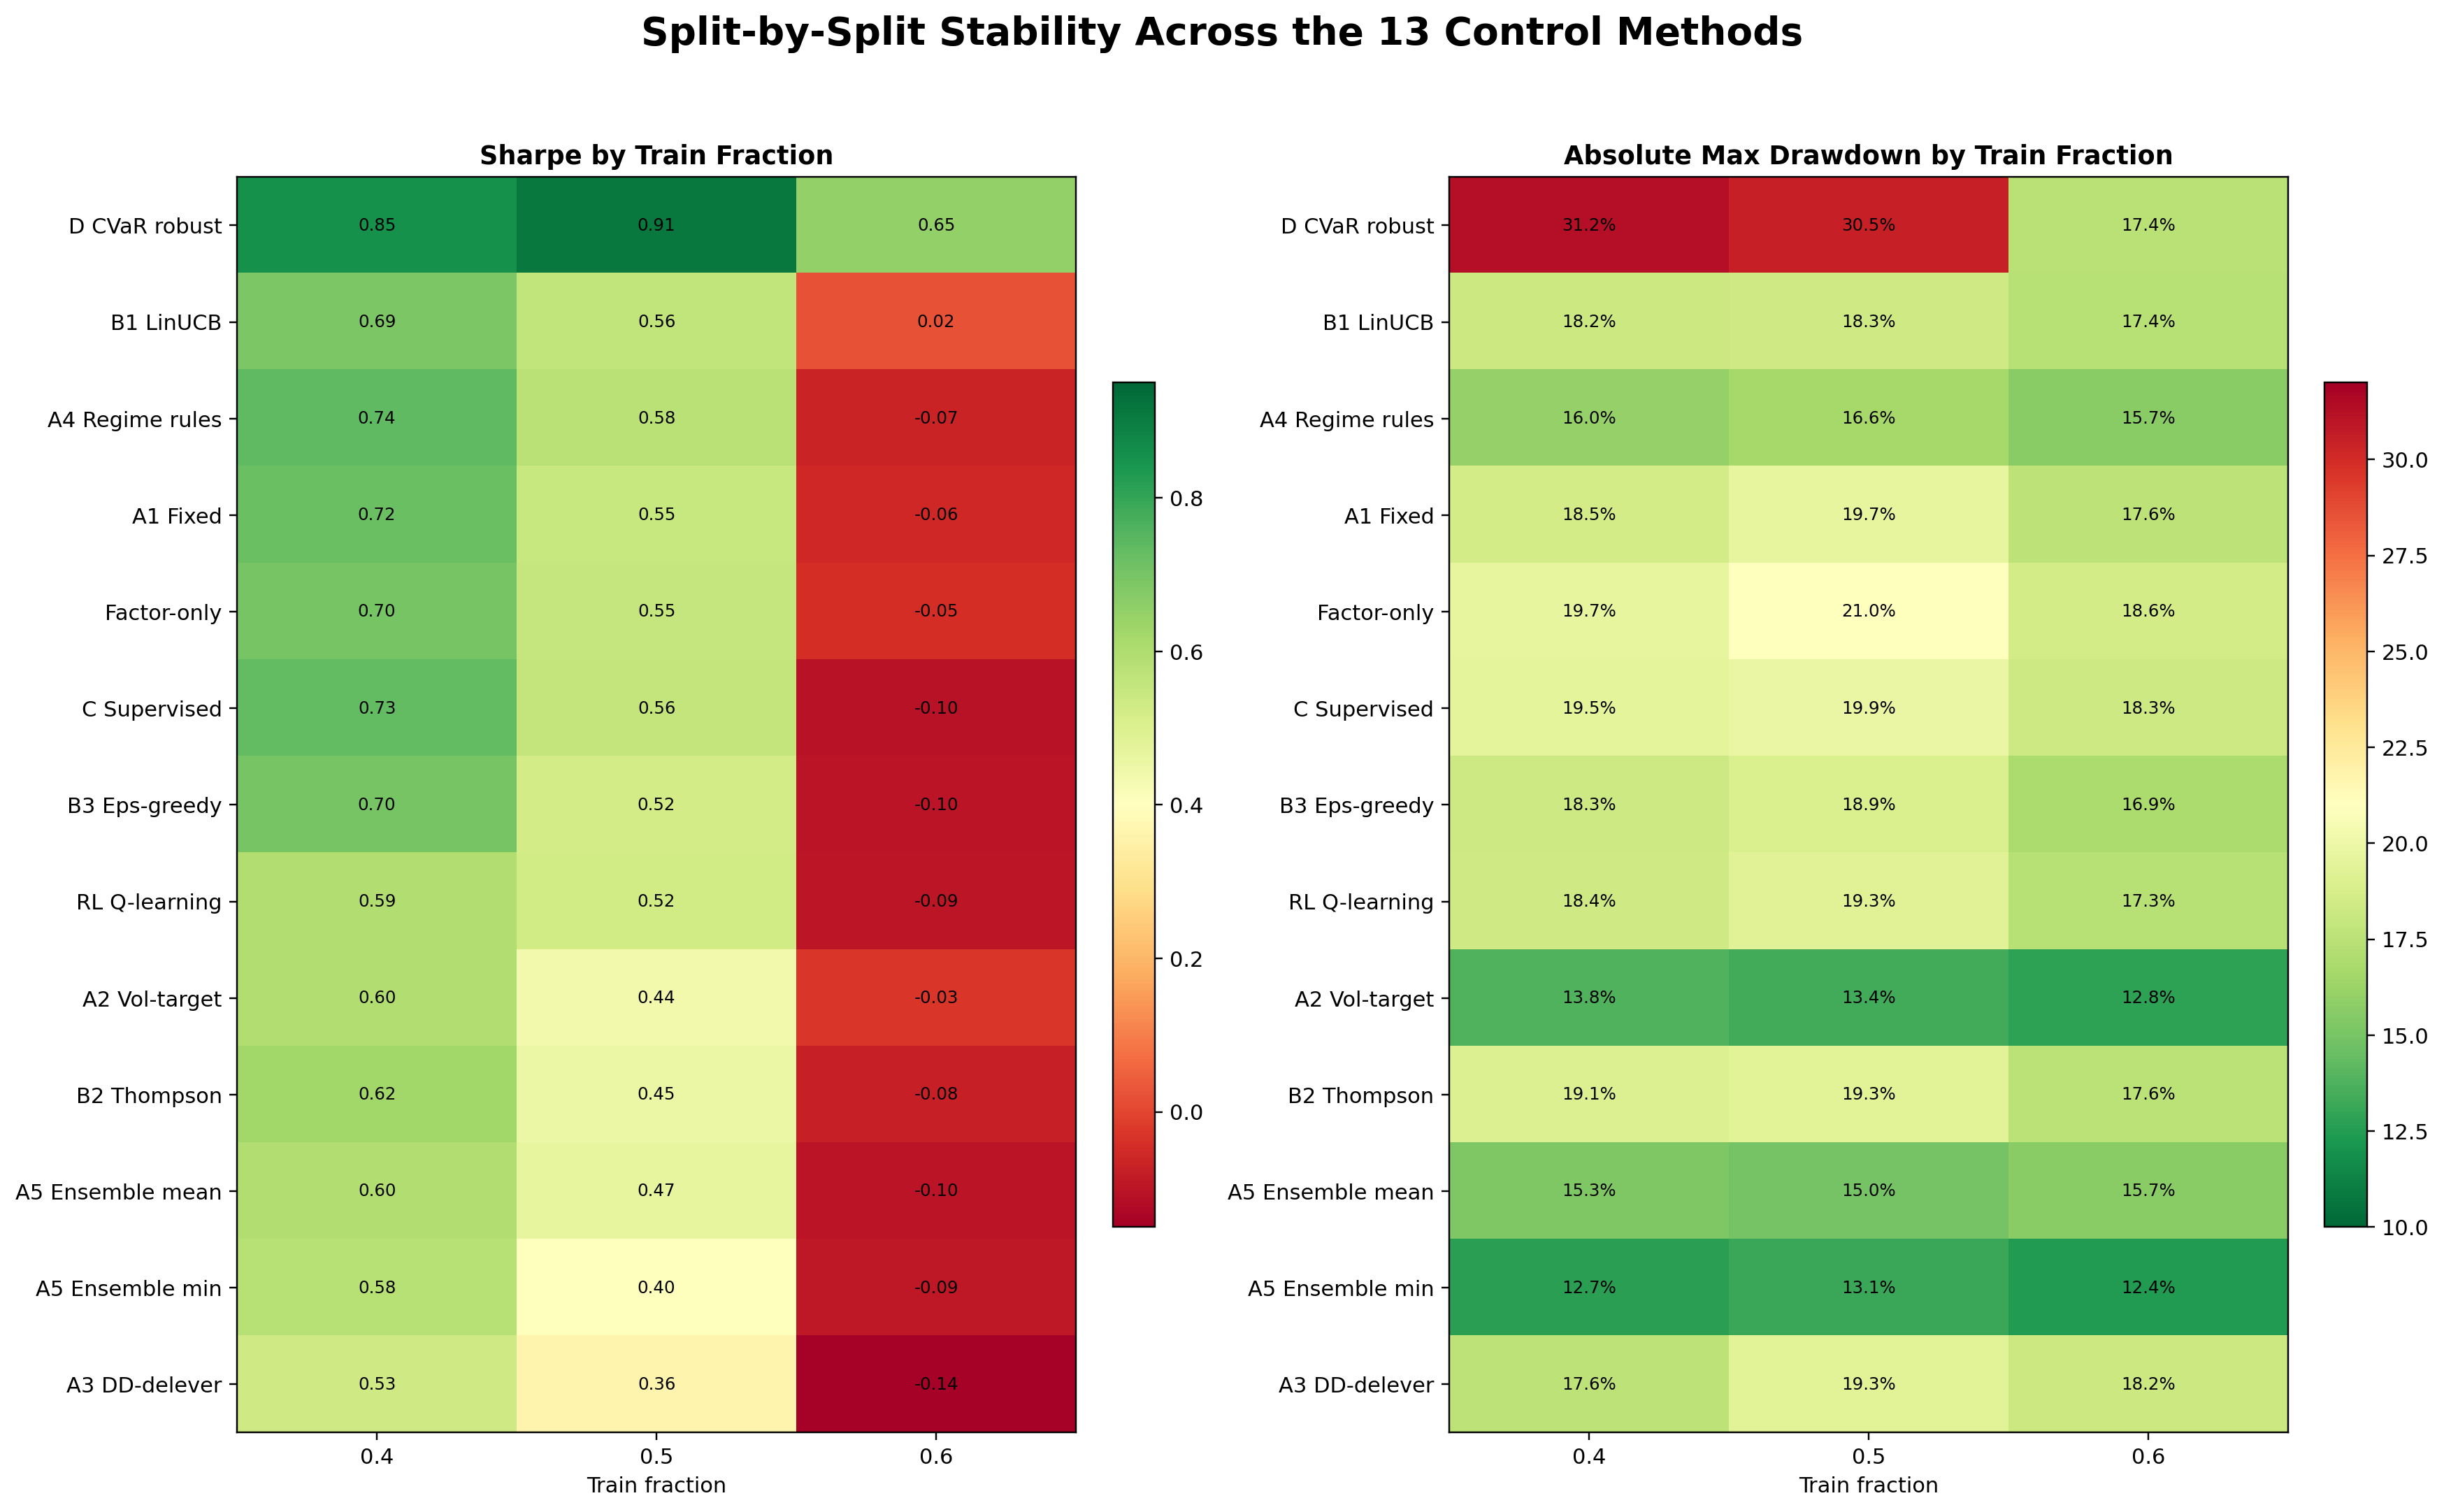
\includegraphics[width=\textwidth]{../../control_split_heatmaps.png}
\caption{Split-by-split stability across the 13 control methods. The left panel
shows Sharpe by train fraction; the right panel shows absolute maximum drawdown.
The figure highlights both the breadth of the CVaR-robust point-estimate lead
and the fact that it does not dominate every downside metric, especially
realized maximum drawdown.}
\label{fig:control_heatmaps}
\end{figure*}
}{
\noindent\textit{Research note.} The plot generator also emits a split-stability
heatmap for the control-comparison suite.
}

\subsection{Legacy Ablation and Complexity Pruning}

The control-comparison headline does not make the legacy ablation evidence
irrelevant. On the contrary, the ablation table explains why the architecture
was revised in the first place. It asks whether the old RL-heavy stack was
actually earning its complexity before the broader controller comparison was
run. The \emph{factor-only benchmark} row in Table~\ref{tab:ablation_summary}
belongs to this legacy ablation suite and is therefore not directly comparable
to the factor-only baseline in Table~\ref{tab:metrics}; the two tables summarize
different archived suites with different purposes.

\begin{table*}[t]
\centering
\caption{Legacy ablation summary across train/test split settings. The
factor-only row belongs to the archived pruning suite used to diagnose the old
RL-heavy stack and is not directly comparable to the control-comparison
factor-only baseline in Table~\ref{tab:metrics}.}
\label{tab:ablation_summary}
\begingroup\small
\begin{tabular}{@{} l r r r r r @{}}
\toprule
\textbf{Component} & \textbf{Return} & \textbf{Vol.} & \textbf{Sharpe} & \textbf{Max DD} & \textbf{Calmar} \\
\midrule
Factor-only benchmark       & 20.2\% & 19.8\% & 0.82 & $-$27.6\% & 0.74 \\
Alpha stack (fixed weights) & 9.9\%  & 13.4\% & 0.45 & $-$19.4\% & 0.51 \\
Alpha stack (adaptive)      & 9.2\%  & 13.4\% & 0.40 & $-$19.6\% & 0.46 \\
Portfolio RL (fixed alpha)  & 7.8\%  & 12.1\% & 0.32 & $-$17.5\% & 0.44 \\
Full pipeline (fixed alpha) & 7.9\%  & 12.2\% & 0.33 & $-$18.1\% & 0.43 \\
Full pipeline               & 7.3\%  & 12.0\% & 0.29 & $-$17.4\% & 0.42 \\
\bottomrule
\end{tabular}
\endgroup
\end{table*}

\IfFileExists{../../legacy_pruning_story.png}{
\begin{figure*}[t]
\centering
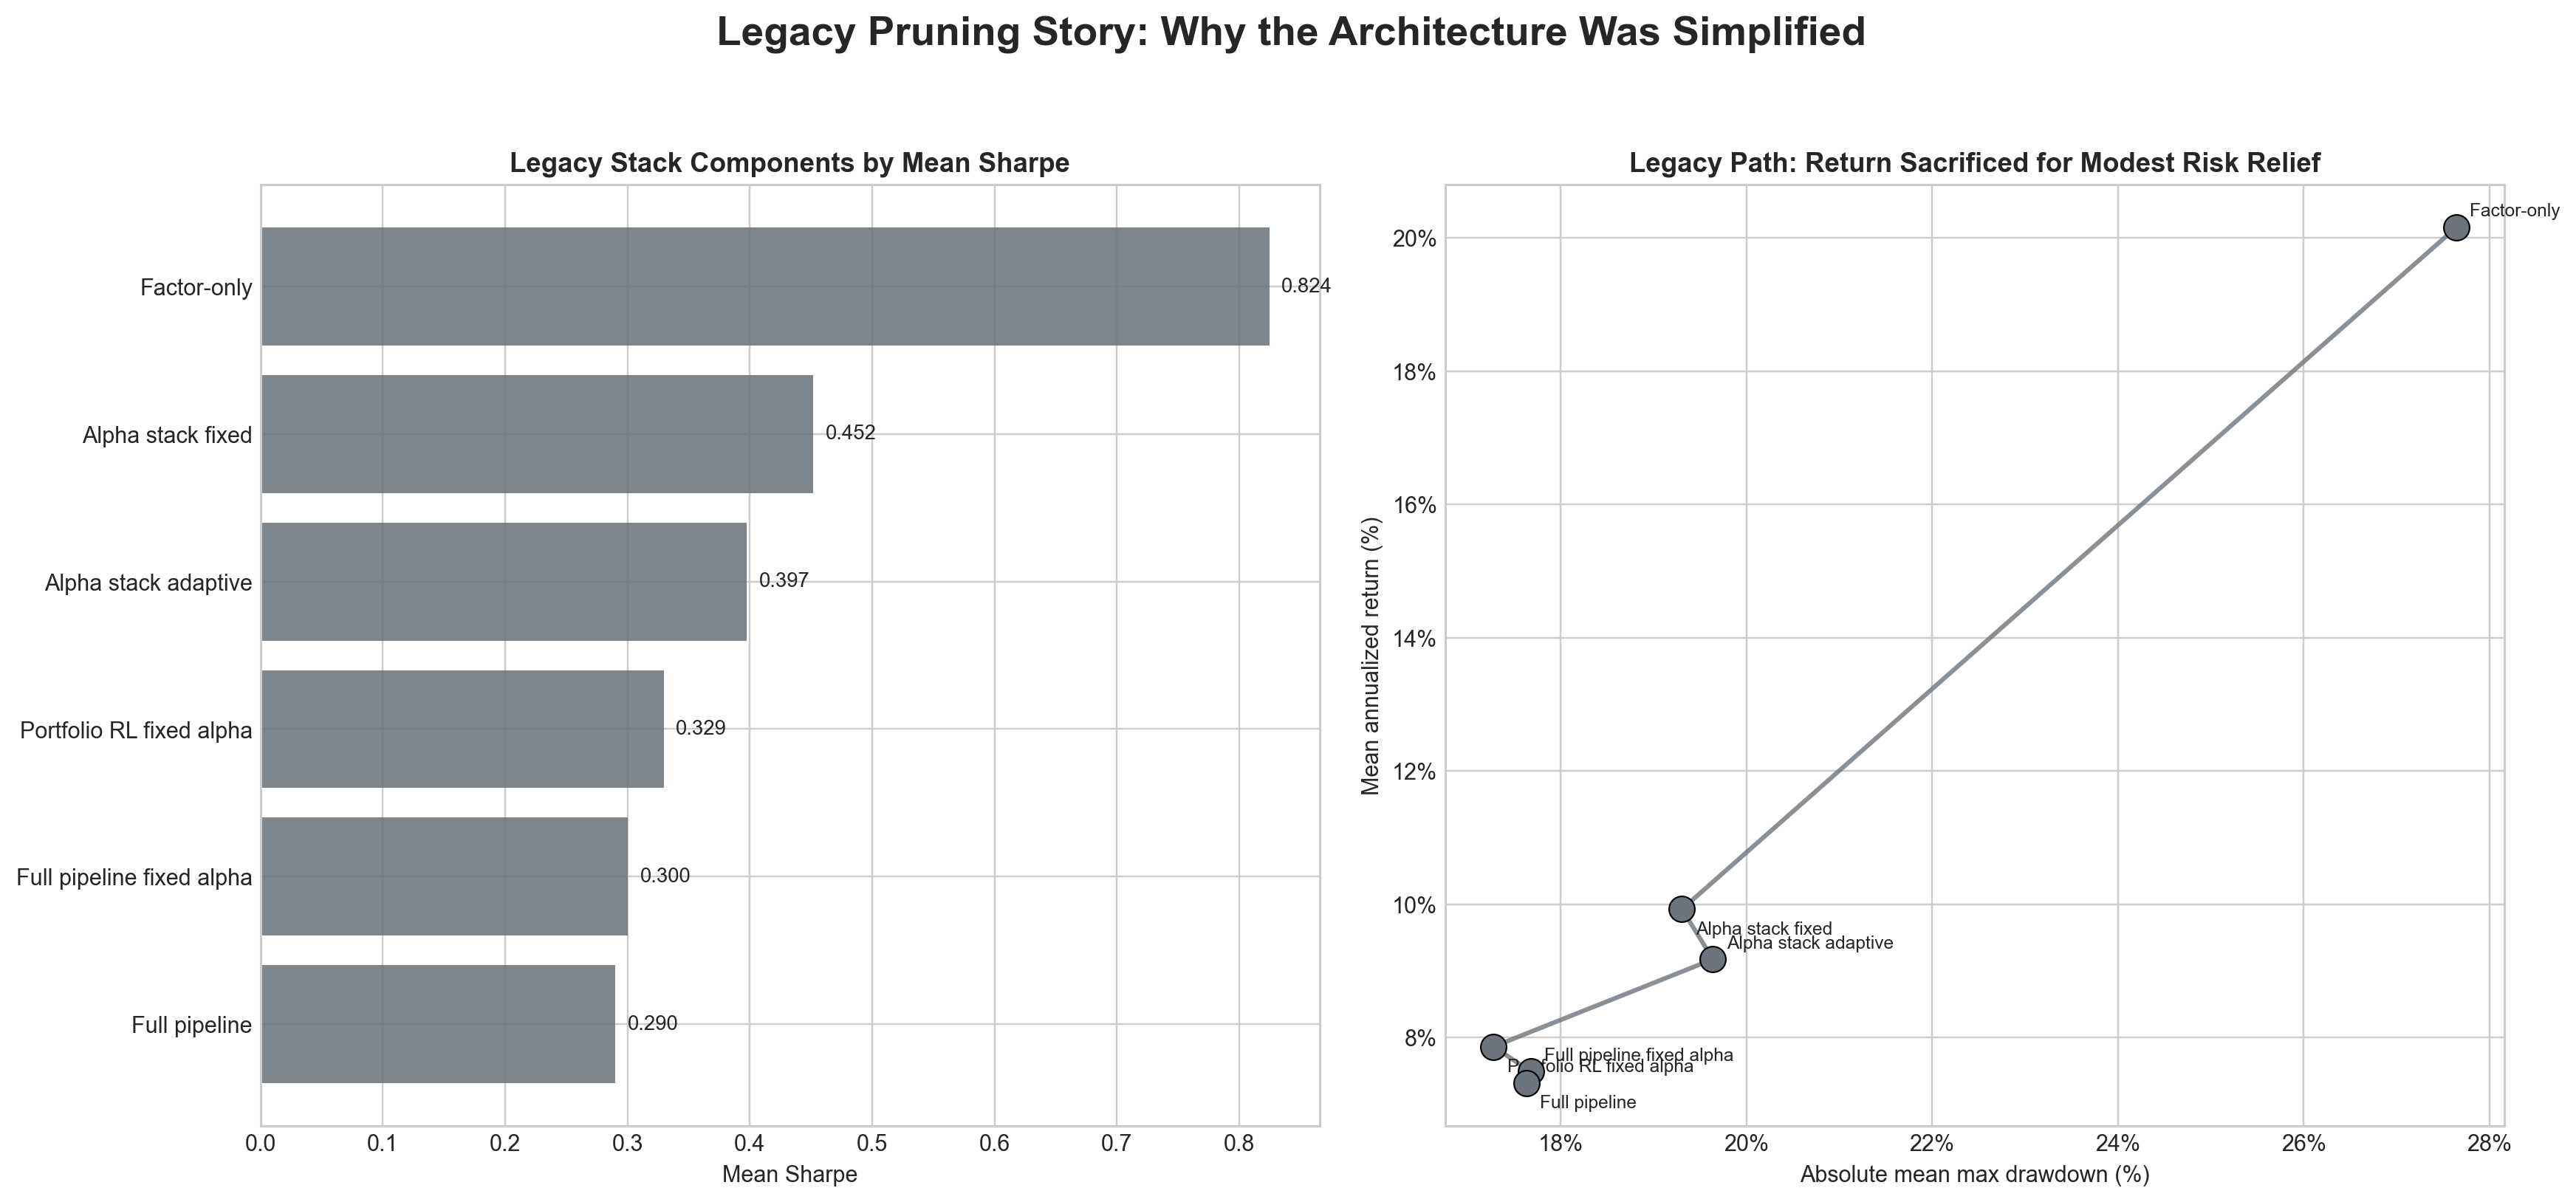
\includegraphics[width=\textwidth]{../../legacy_pruning_story.png}
\caption{Legacy pruning story from the retained ablation suite. The left panel
orders the old architecture variants by mean Sharpe; the right panel shows the
pruning path in return-versus-drawdown space. Its role in the revised paper is
diagnostic: it explains why the study moved away from defending the old RL
stack and toward a broader control-method comparison.}
\label{fig:legacy_pruning}
\end{figure*}
}{}

\begin{table}[t]
\centering
\caption{Rolling-window robustness summary for the full pipeline.}
\label{tab:robustness_summary}
\begingroup\small
\begin{tabular}{@{} >{\raggedright\arraybackslash}p{0.70\columnwidth} r @{}}
\toprule
\textbf{Statistic} & \textbf{Value} \\
\midrule
Rolling windows                                    & 6 \\
Median full-pipeline Sharpe                        & 0.59 \\
Median full-pipeline Calmar                        & 1.07 \\
Median full-pipeline Max DD                        & $-$8.9\% \\
Frac. windows full beats factor-only benchmark on drawdown & 67\% \\
Frac. windows full beats factor-only benchmark on Calmar   & 17\% \\
Frac. windows full beats SPY on Sharpe             & 17\% \\
Frac. windows full beats SPY on Calmar             & 17\% \\
\bottomrule
\end{tabular}
\endgroup
\end{table}

The ablation story remains sharply negative for the old learned stack. Averaged
across split settings, the factor-only benchmark reaches mean Sharpe 0.82,
whereas the legacy full pipeline reaches only 0.29. Fixed alpha combination is
stronger than adaptive combination, and every additional learned layer beyond
the factor core lowers average Sharpe materially. This is exactly the pruning
result that motivated the shift from an RL-centric paper to a control-method
comparison paper.

\noindent\textit{Implication for RQ3.} The old RL-heavy complexity is not
justified. The factor core is the credible source of alpha, and the original
full pipeline is best interpreted as a negative control that motivated the
revised study.

\subsection{Legacy Full-Pipeline Reference and Significance}

The old full pipeline is retained as a secondary reference because it anchors
the transition from the earlier project narrative to the new one. In the
refreshed root-level confidence-interval artifact, its point estimates are
9.0\% annualized return, 0.423 Sharpe, 0.459 Calmar, and $-$19.6\% maximum
drawdown.

The bootstrap significance summary in Table~\ref{tab:legacy_bootstrap_significance}
shows that this legacy full pipeline is significantly worse than the
factor-only benchmark on Sharpe and annualized return, significantly worse than
vol-targeting on both dimensions, and materially weaker than
drawdown-deleveraging on annualized return. It is not statistically
distinguishable from SPY or end-to-end PPO on Sharpe in the completed bundle.

\begin{table*}[t]
\centering
\caption{Block-bootstrap significance for the legacy full pipeline versus
selected baselines (Sharpe deltas).}
\label{tab:legacy_bootstrap_significance}
\small
\begin{tabular}{@{} p{0.42\textwidth} r r r @{}}
\toprule
\textbf{Comparison} & \textbf{Delta Sharpe} & \textbf{95\% CI} & \textbf{p-value} \\
\midrule
Full -- SPY                   & -0.16 & [-0.91, 0.51] & 0.615 \\
Full -- Factor-only benchmark & -0.58 & [-1.14, -0.15] & 0.005 \\
Full -- Vol-target            & -0.47 & [-0.98, -0.03] & 0.035 \\
Full -- DD-Delever            & -0.50 & [-1.04, 0.06] & 0.070 \\
Full -- E2E RL (PPO)          & -0.14 & [-1.19, 0.81] & 0.820 \\
\bottomrule
\end{tabular}
\end{table*}

The Jobson--Korkie summary tells the same story more narrowly: the legacy full
pipeline is significantly worse than the factor benchmark on Sharpe at the
5\% level, while differences versus SPY, PPO, and the stronger rule baselines
are not statistically decisive. So even as a legacy reference, the old RL
branch does not recover the central economic claim.

\subsection{Reward Sensitivity and Robustness of the Legacy Branch}

Reward design affects where the retained full-pipeline controller lands on the
risk-return frontier, but only within a relatively narrow band. Across the
reward-function ablation, the Sortino reward is best for the legacy branch,
reaching about 9.1\% annualized return and 0.44 Sharpe, while the broader
ranking versus factor-only, rules, and robust optimization is unchanged.

\begin{table}[t]
\centering
\small
\caption{Reward-function ablation for the full pipeline on the revised bundle.}
\label{tab:reward_ablation}
\begin{tabular}{@{} l r r r r @{}}
\toprule
\textbf{Reward} & \textbf{Return} & \textbf{Sharpe} & \textbf{Max DD} & \textbf{Calmar} \\
\midrule
Differential Sharpe & 9.3\% & 0.45 & $-$17.0\% & 0.55 \\
Return              & 9.5\% & 0.48 & $-$17.2\% & 0.55 \\
Sortino             & 9.5\% & 0.48 & $-$17.0\% & 0.56 \\
Mean-Variance       & 9.2\% & 0.45 & $-$17.8\% & 0.52 \\
\bottomrule
\end{tabular}
\end{table}

The rolling-window and time-series cross-validation diagnostics remain useful,
but they should now be read as diagnostics for the retained legacy branch, not
as the main source of the paper's contribution. The rolling-window summary
shows median full-pipeline Sharpe 0.59, median Calmar 1.09, and median maximum
drawdown $-$8.9\%. The corresponding benchmark-beat fractions remain weak:
the legacy full pipeline beats SPY on Sharpe in only 17\% of windows and beats
the factor benchmark on Calmar in only 17\% of windows. The blocked time-series
CV summary is similarly modest, with Sharpe 0.41 $\pm$ 0.57 and Calmar
0.72 $\pm$ 0.51 across five folds.

\noindent\textit{Implication for the overall claim.} The legacy branch still
does not show a structural edge. Its main value in the revised paper is as a
transparent negative result that motivated the broader controller comparison.

\IfFileExists{../../pipeline_rolling_windows.png}{
\begin{figure*}[t]
\centering
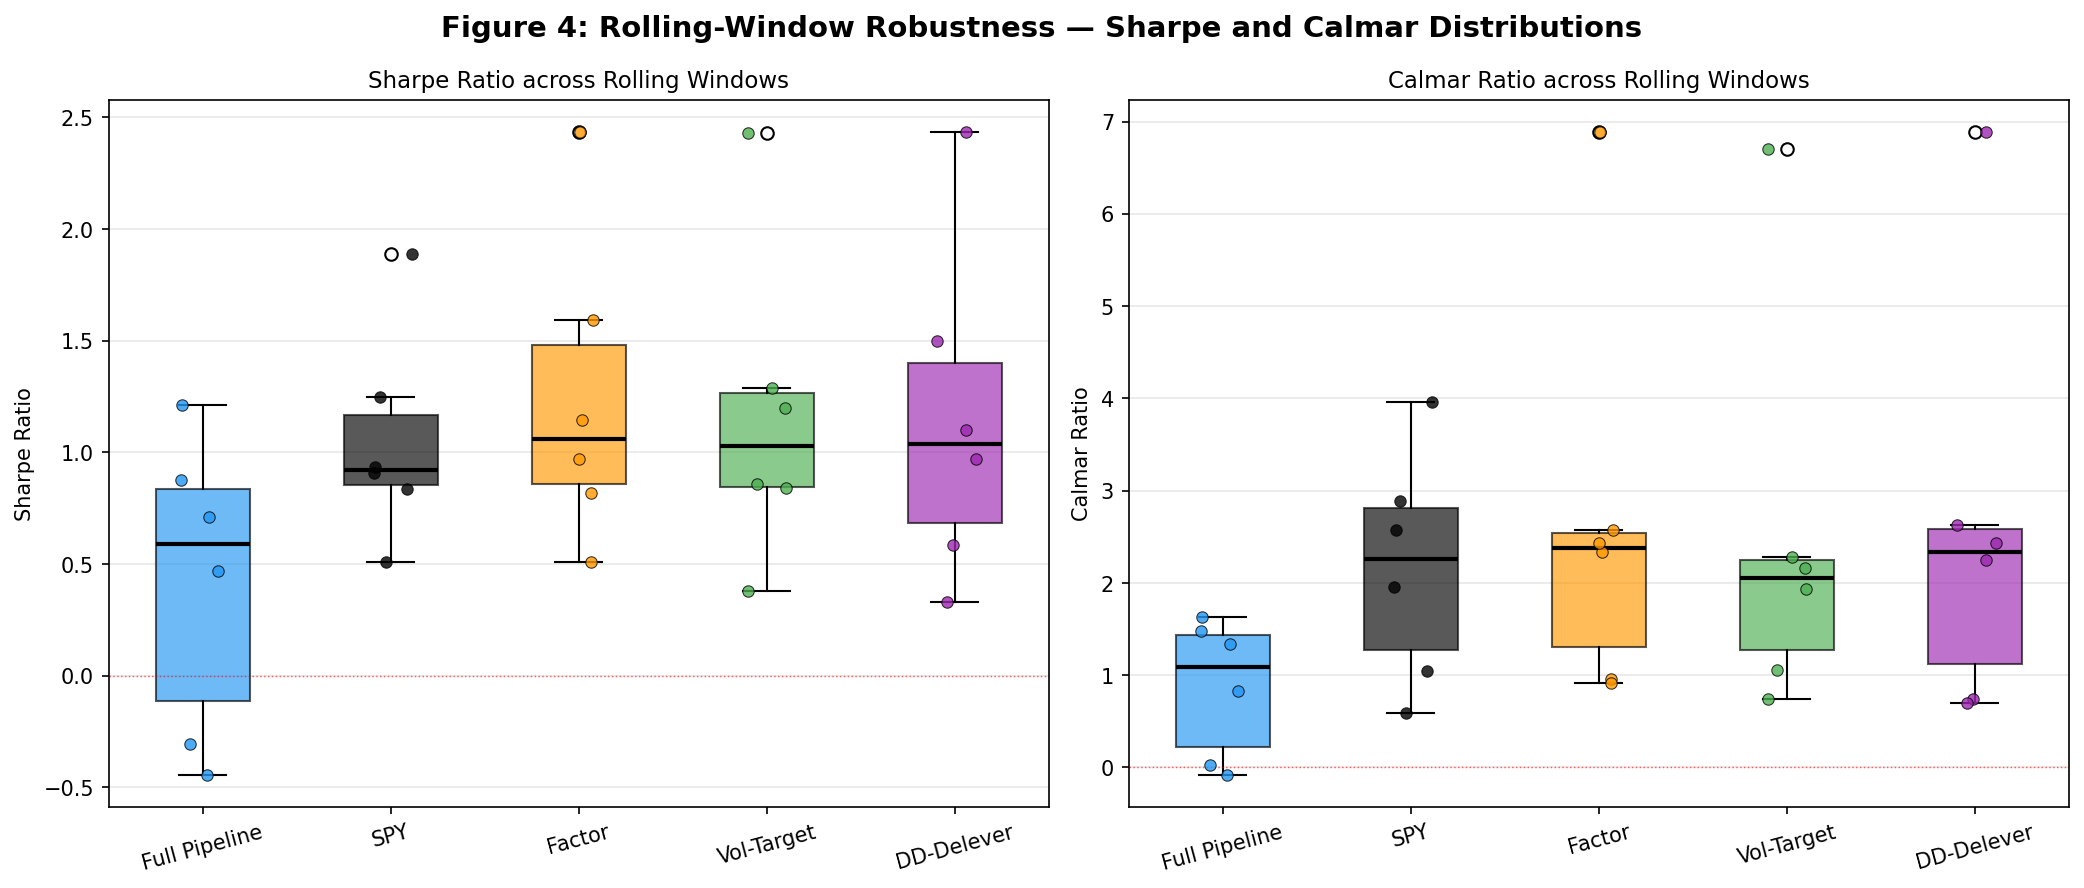
\includegraphics[width=\textwidth]{../../pipeline_rolling_windows.png}
\caption{Rolling-window robustness for the retained legacy full pipeline. The
pattern remains mixed: drawdown improves more often than Sharpe, and the
windows should be interpreted as internal robustness slices from one
historical sample rather than independent replications.}
\label{fig:rollingwindows}
\end{figure*}
}{}

\section{Discussion}

The experimental results support three conclusions of methodological importance.

First, the control-mechanism comparison has a strongest point-estimate winner.
CVaR-aware robust optimization leads the finished suite by a wide margin,
reaching mean Sharpe 0.81 versus 0.40 for the factor-only baseline and 0.42
for the best learner, LinUCB. In other words, once the factor, GARCH, and HMM
alpha engine is fixed, the biggest incremental value comes from explicit
downside-aware optimization rather than from additional sequential-learning
complexity. This does not mean it dominates every risk lens: it also has the
deepest mean maximum drawdown in the control-comparison table, which is a
reminder that CVaR control and realized pathwise drawdown are not the same
objective.

Second, simple rules are stronger than a complexity-first story would suggest.
Regime-aware rules reach 0.415 mean Sharpe with better maximum drawdown than
the factor-only baseline, while fixed exposure and volatility targeting provide
clean, interpretable trade-offs between participation and protection. This is a
useful empirical result in its own right: the paper does not need learned
control to justify itself, because a disciplined comparison already shows that
simple rules can be credible, competitive baselines.

Third, the learning-based methods are mixed rather than dominant. LinUCB is the
best learner and does slightly improve on the factor-only baseline, but the
bandits, supervised controller, and Q-learning RL all remain well below the
robust optimizer on risk-adjusted performance. That negative result is not an
embarrassment; it is part of the methodological contribution. The point of the
revised paper is to delimit where learning helps and where simpler or more
structured controllers remain stronger.

What did not work is therefore just as informative as what did. The old
RL-heavy stack still collapses in the legacy ablation table. Drawdown-based
deleveraging is weaker than the better simple rules. Ensemble rules are more
stable than exciting. The learning methods adapt, but they do not earn a clear
performance premium in this daily U.S.-equity setting. These failures are
precisely what turn the project from a prototype report into a more credible
control-method study.

\subsection{When Practitioners Should Use Which Control Style}

The archived evidence suggests three practical regimes of use. If the main
objective is to maximize risk-adjusted performance on top of an already strong
factor engine, the current bundle points toward CVaR-aware robust optimization.
It is the only method that is clearly stronger across mean Sharpe, return, and
Calmar in the completed comparison.

If simplicity, interpretability, and implementation speed matter more than
squeezing out every last point estimate, regime-aware rules are the strongest
practical baseline. They improve drawdown materially, remain easy to explain,
and do not require the extra tuning burden associated with bandits or RL.

The learning-based methods are still useful as research instruments, but not as
the default recommendation from this bundle. LinUCB suggests that lightweight
adaptation can be competitive, and the supervised controller is not far behind,
yet neither closes the gap to robust optimization. The practical contribution
is therefore not ``always use learning.'' It is to compare structured rules,
learning, and robust optimization over a shared alpha engine before accepting
additional controller complexity.

\section{Threats to Validity and Future Work}

The implementation remains research code, and several caveats apply. Macro
inputs are shifted by a configurable lag, but they are not full vintage series
with revision-aware histories. SEC enrichment can be used as a static
cross-sectional prior, but it still does not constitute a true point-in-time
fundamentals database. Transaction costs are more realistic than before, yet
they remain stylized rather than venue-specific. The robustness engine still
depends on one underlying historical sample even when it slices that sample in
multiple ways.

Several additional threats deserve explicit acknowledgement. First, the design
has been iterated by observing backtest behavior, which raises the possibility
of researcher degrees of freedom even when each individual change is motivated.
Second, the traded universe is broader than in the earlier prototype but still
narrow relative to institutional equity universes, so the results may depend
partly on the selected names. Third, daily data are appropriate for a medium-
horizon allocation study but cannot validate intraday execution claims. Finally,
the project deliberately leans on free or public data sources, which improves
accessibility but necessarily limits point-in-time fidelity and market
microstructure realism.

A further caveat is benchmark fairness: although the rule-based and PPO
baselines are designed to be strong and informative, their exact specification
still influences comparative conclusions. Because the evaluation suite reports
many metrics and comparator strategies, some apparent wins and losses should
also be interpreted with the usual caution around multiple comparisons.
External validity is also limited: conclusions drawn from a daily U.S.-equity
allocation setting may not transfer unchanged to other asset classes,
frequencies, or market microstructure regimes.

The currently reported robustness summary is still based on only six rolling
windows, five blocked time-series CV folds, and one underlying historical
sample. The workshop interpretation should therefore be that the robustness
engine is now part of the methodology, not that robustness has been exhaustively
established across many independent market environments. A further limitation
of the current artifact bundle is that the pairwise uncertainty analysis is
strongest for the legacy full pipeline versus baselines; the paper does not yet
report equally thorough bootstrap comparisons among the new winner
\texttt{D\_cvar\_robust} and the strongest alternative controllers such as
regime-aware rules and LinUCB.

Natural next steps follow directly from this new result. The highest-value
extensions are pairwise significance tests across the new controller families,
broader universes and asset classes, stricter point-in-time data treatment,
more systematic benchmark tuning, and deeper learned-controller baselines such
as modern deep RL used purely as control-layer comparators. If protection
overlays re-enter the stack later, they should do so as separately validated
extensions rather than as assumed core architecture.

\section{Conclusion}

This paper reframes the project from an RL question into a broader empirical
comparison of control mechanisms for factor-based portfolio management. The
shared finance-first alpha engine remains modular and interpretable; the main
scientific question is which controller adds the most value once that engine is
already in place.

The completed frozen bundle gives a clear answer. CVaR-aware robust
optimization is the strongest point-estimate controller in the study, simple
regime-aware rules are the best practical baseline, and the learning-based
methods do not beat the optimization-based approach. Equally importantly, the
paper leaves behind a frozen-bundle evaluation protocol that can support
future controller comparisons under a consistent empirical standard. In the
reported sample, the evidence supports uncertainty-aware robust optimization as
the strongest point-estimate control layer and rejects the stronger claim that
additional learning complexity is necessary for daily portfolio rebalancing.

\appendix

\section{Implementation Snapshot}

\subsection{Revised-Study Snapshot}

The revised frozen bundle reported in the paper corresponds to the simplified
finance-first stack summarized in Table~\ref{tab:archsnapshot}. The most
important change relative to the earlier project versions is that the paper now
evaluates a family of controllers on top of the same allocator rather than
trying to defend one learned controller in isolation.

\begin{table*}[t]
\centering
\caption{Active study design in the revised frozen bundle.}
\label{tab:archsnapshot}
\small
\begin{tabular}{@{} l p{0.72\textwidth} @{}}
\toprule
\textbf{Layer} & \textbf{Active design} \\
\midrule
Alpha layer & Factor, GARCH, and HMM sleeves only \\
Combiner & Adaptive IC-weighted combiner with fixed-weight ablation \\
Allocator & Long-only, capped, turnover-penalized, factor-anchored target book \\
Controller candidates & Factor-only baseline, simple rules, ensembles, contextual bandits, supervised control, CVaR-aware robust optimization, and Q-learning RL \\
Execution & No-trade band plus three-part transaction-cost model \\
Legacy reference branch & RL-heavy full pipeline, PPO comparator, and pruning ablations retained as negative-reference evidence \\
\bottomrule
\end{tabular}
\end{table*}

\subsection{Research Artifacts}

For the revised root-level run discussed in the paper, the research runner
writes the artifacts below into the repository root alongside the paper outputs:
\begin{enumerate}[leftmargin=1.5em, itemsep=2pt, topsep=4pt]
\item \texttt{research\_metrics.csv}: tabular output for ablation and robustness runs;
\item \texttt{research\_control\_comparison.csv}: split-aggregated controller comparison across the 13 evaluated methods;
\item \texttt{research\_ablation\_summary.csv}: split-aggregated ablation summaries;
\item \texttt{research\_robustness\_summary.csv}: rolling-window medians and benchmark beat fractions;
\item \texttt{research\_regime\_summary.csv}: regime-conditioned action, turnover, and return summaries;
\item \texttt{research\_rolling\_references.csv}: rolling benchmark metrics for SPY and the factor-only benchmark;
\item \texttt{research\_bootstrap\_cis.csv}: block-bootstrap confidence intervals for key strategy metrics;
\item \texttt{research\_bootstrap\_significance.csv}: pairwise bootstrap deltas and $p$-value summaries versus benchmark strategies;
\item \texttt{research\_jobson\_korkie.csv}: parametric Sharpe-ratio comparison tests;
\item \texttt{research\_ts\_cv.csv}: blocked time-series cross-validation summaries;
\item \texttt{research\_summary.json}: serialized configuration and best-per-suite summaries; and
\item \texttt{pipeline\_research\_eval.png}: compact paper-facing summary figure;
\item \texttt{pipeline\_rolling\_windows.png}: rolling-window robustness figure; and
\item \texttt{pipeline\_reward\_ablation.png}: reward-ablation figure.
\end{enumerate}

Together with the feature-availability contract embedded in each backtest run,
these artifacts make it easier to compare results across alternative timing,
cost, and control assumptions without manually reconstructing the experimental
context after the fact.

\subsection{Supplementary Diagnostic Figures}

These figures are diagnostic and illustrative; the primary evidentiary claims
of the paper rest on Tables~\ref{tab:metrics}--\ref{tab:legacy_bootstrap_significance}
and Figures~\ref{fig:control_overview}, \ref{fig:control_heatmaps},
\ref{fig:legacy_pruning}, and \ref{fig:rollingwindows}. The appendix
intentionally focuses on figures produced directly by the revised root-level
bundle and omits older dashboards that are not tied to the reported evidence.

\IfFileExists{../../pipeline_reward_ablation.png}{
\begin{figure*}[t]
\centering
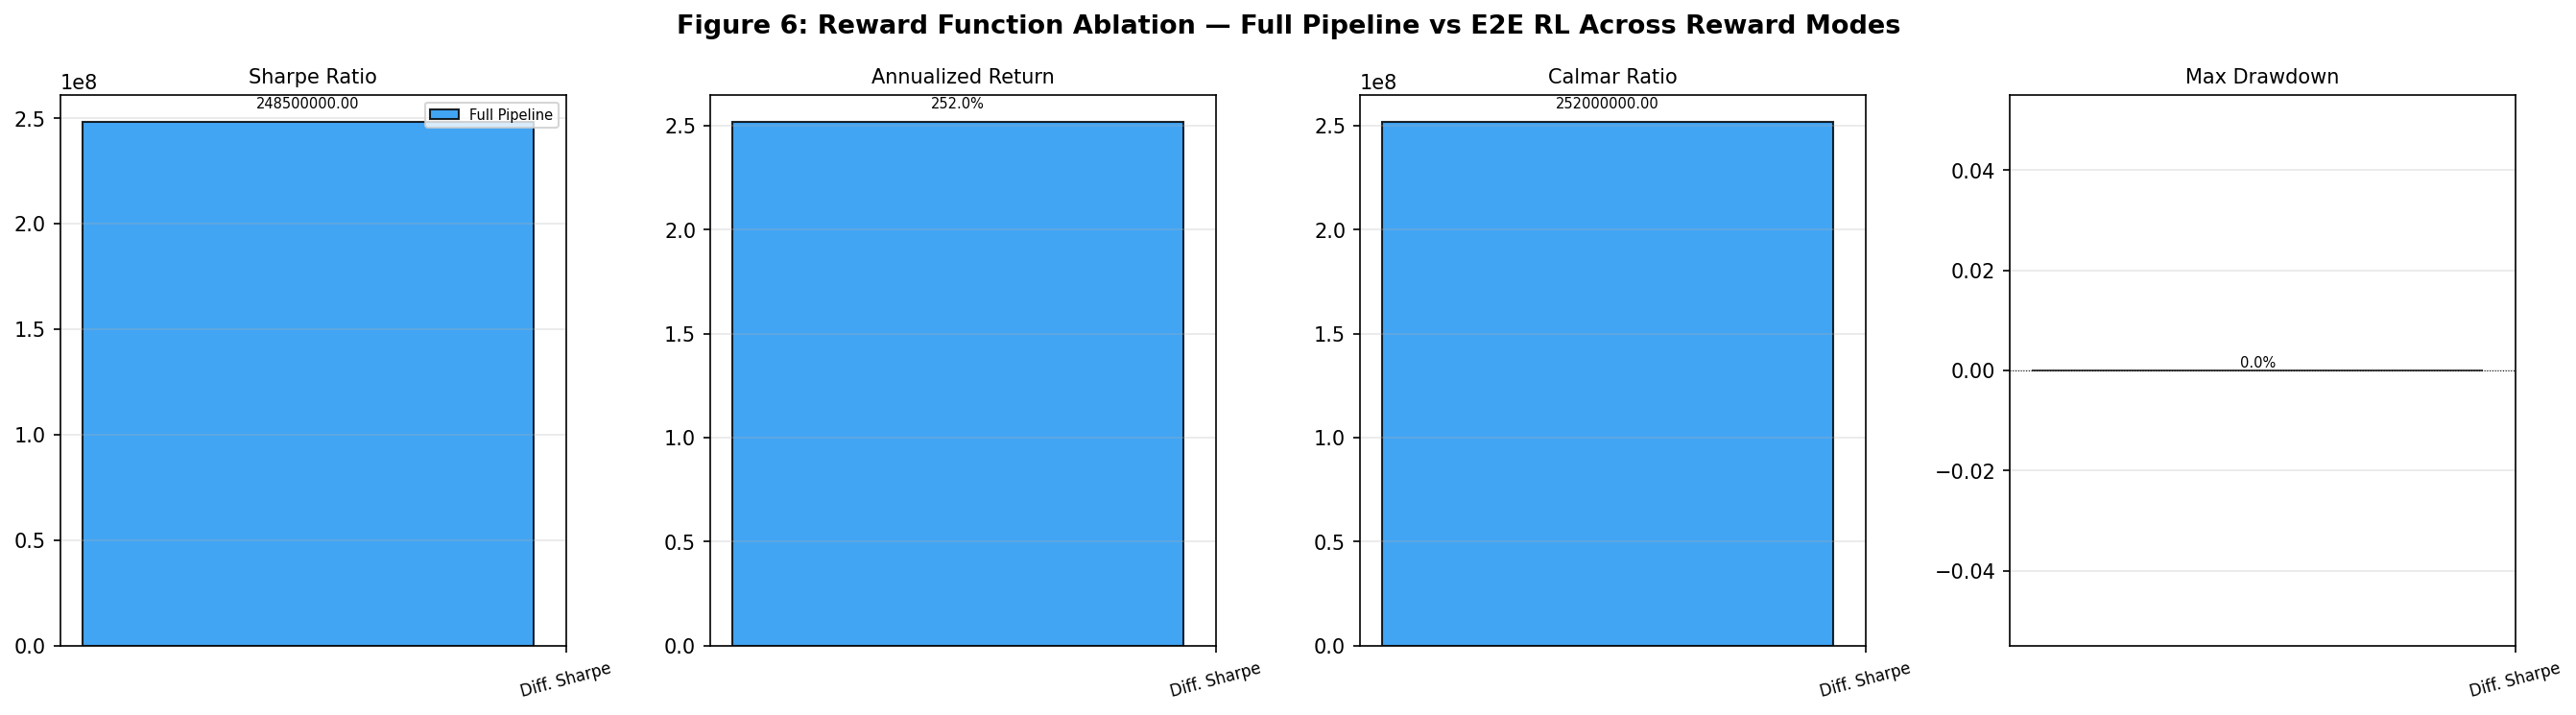
\includegraphics[width=\textwidth]{../../pipeline_reward_ablation.png}
\caption{Supplementary reward-ablation figure for the revised bundle. Reward
choice changes the controller's operating point modestly, but the broader
ranking versus the factor-only benchmark and the strongest rule-based overlays
is unchanged.}
\label{fig:rewardfig}
\end{figure*}
}{}

\begin{thebibliography}{99}

\bibitem{almgren2000}
R. Almgren and N. Chriss.
\newblock Optimal execution of portfolio transactions.
\newblock \emph{Journal of Risk}, 3(2):5--39, 2000.

\bibitem{buehler2019}
H. Buehler, L. Gonon, J. Teichmann, and B. Wood.
\newblock Deep hedging.
\newblock \emph{Quantitative Finance}, 19(8):1271--1291, 2019.

\bibitem{bollerslev1986}
T. Bollerslev.
\newblock Generalized autoregressive conditional heteroskedasticity.
\newblock \emph{Journal of Econometrics}, 31(3):307--327, 1986.

\bibitem{chen2021}
L. Chen, M. Pelger, and J. Zhu.
\newblock Deep learning in asset pricing.
\newblock \emph{SSRN Working Paper 3350138}, revised 2021.

\bibitem{cong2021}
Y. Cong, B. Deng, X. Bao, and H. Dai.
\newblock AlphaPortfolio: Direct construction through deep reinforcement learning
  and interpretable representation learning.
\newblock \emph{Proceedings of the AAAI Conference on Artificial Intelligence},
  35(6):4831--4839, 2021.

\bibitem{deng2017}
Y. Deng, F. Bao, Y. Kong, Z. Ren, and Q. Dai.
\newblock Deep direct reinforcement learning for financial signal representation
  and trading.
\newblock \emph{IEEE Transactions on Neural Networks and Learning Systems},
  28(3):653--664, 2017.

\bibitem{du2020}
Y. Du, P. N. Kolm, A. Ritter, and T. Wang.
\newblock Deep reinforcement learning for option replication and hedging.
\newblock \emph{The Journal of Financial Data Science}, 2(4):44--59, 2020.

\bibitem{engle1982}
R. F. Engle.
\newblock Autoregressive conditional heteroscedasticity with estimates of the
  variance of United Kingdom inflation.
\newblock \emph{Econometrica}, 50(4):987--1007, 1982.

\bibitem{engle1987}
R. F. Engle and C. W. J. Granger.
\newblock Co-integration and error correction: representation, estimation, and
  testing.
\newblock \emph{Econometrica}, 55(2):251--276, 1987.

\bibitem{fama1993}
E. F. Fama and K. R. French.
\newblock Common risk factors in the returns on stocks and bonds.
\newblock \emph{Journal of Financial Economics}, 33(1):3--56, 1993.

\bibitem{giglio2022}
S. Giglio, D. Xiu, and D. Zhang.
\newblock Machine learning in asset pricing.
\newblock \emph{Annual Review of Financial Economics}, 14:337--368, 2022.

\bibitem{gu2020}
S. Gu, B. Kelly, and D. Xiu.
\newblock Empirical asset pricing via machine learning.
\newblock \emph{Review of Financial Studies}, 33(5):2223--2273, 2020.

\bibitem{hamilton1989}
J. D. Hamilton.
\newblock A new approach to the economic analysis of nonstationary time series
  and the business cycle.
\newblock \emph{Econometrica}, 57(2):357--384, 1989.

\bibitem{jander2025}
J. Jander, H. H. Li, M. Schmid, and T. Pohl.
\newblock Reinforcement learning in finance: From current practice to standards
  and benchmarks.
\newblock \emph{SSRN Working Paper 5703882}, 2025.

\bibitem{jegadeesh1993}
N. Jegadeesh and S. Titman.
\newblock Returns to buying winners and selling losers: implications for stock
  market efficiency.
\newblock \emph{Journal of Finance}, 48(1):65--91, 1993.

\bibitem{jiang2017}
Z. Jiang, D. Xu, and J. Liang.
\newblock A deep reinforcement learning framework for the financial portfolio
  management problem.
\newblock \emph{arXiv preprint arXiv:1706.10059}, 2017.

\bibitem{kolm2019}
P. N. Kolm and G. Ritter.
\newblock Modern perspectives on reinforcement learning in finance.
\newblock \emph{SSRN Working Paper 3449401}, 2019.

\bibitem{kolm2019hedge}
P. N. Kolm and G. Ritter.
\newblock Dynamic replication and hedging: A reinforcement learning approach.
\newblock \emph{The Journal of Financial Data Science}, 1(4):159--171, 2019.

\bibitem{moody2001}
J. Moody and M. Saffell.
\newblock Learning to trade via direct reinforcement.
\newblock \emph{IEEE Transactions on Neural Networks}, 12(4):875--889, 2001.

\bibitem{nevmyvaka2006}
Y. Nevmyvaka, Y. Feng, and M. Kearns.
\newblock Reinforcement learning for optimized trade execution.
\newblock In \emph{Proceedings of the 23rd International Conference on Machine
  Learning}, pages 673--680, 2006.

\bibitem{pacheco2023}
D. Pacheco Aznar.
\newblock Portfolio management: A deep distributional reinforcement learning
  approach.
\newblock \emph{SSRN Working Paper 4522084}, 2023.

\bibitem{sun2023}
S. Sun, M. Qin, W. Zhang, H. Xia, C. Zong, J. Ying, Y. Xie, L. Zhao,
  X. Wang, and B. An.
\newblock TradeMaster: A holistic quantitative trading platform empowered by
  reinforcement learning.
\newblock In \emph{Advances in Neural Information Processing Systems 36:
  Datasets and Benchmarks Track}, 2023.

\bibitem{sutton2018}
R. S. Sutton and A. G. Barto.
\newblock \emph{Reinforcement Learning: An Introduction}.
\newblock MIT Press, Cambridge, MA, second edition, 2018.

\bibitem{zhang2020}
Z. Zhang, S. Zohren, and S. Roberts.
\newblock Deep reinforcement learning for trading.
\newblock \emph{The Journal of Financial Data Science}, 2(2):25--40, 2020.

\end{thebibliography}

\end{document}
